\section{Development of the bare metal firmware}
\label{sec:firmware}
This Section describes the development of the bare-metal firmware.

\subsection{Firmware Architecture}
\label{subsec:firmware-arch}
% object dictionary, etc, dependency on RTIC, other things

\begin{figure}[H]
    \centering
    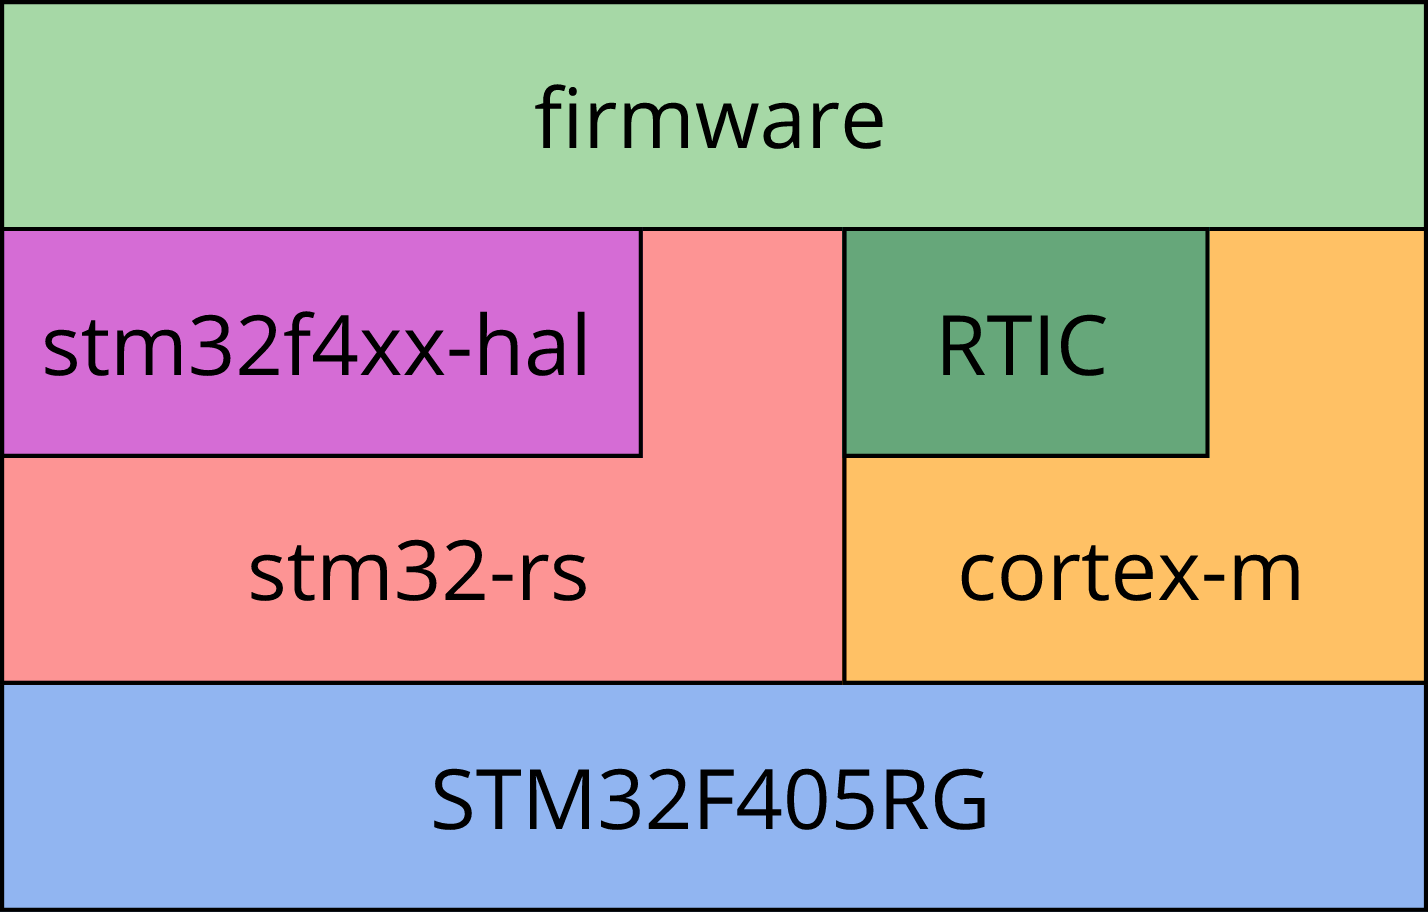
\includegraphics[width=0.5\textwidth]{obrazky/tech_stack}
    \caption{Bare-Metal firmware technology stack.}
    \label{fig:firmware_tech_stack}
\end{figure}

\begin{figure}[H]
    \centering
    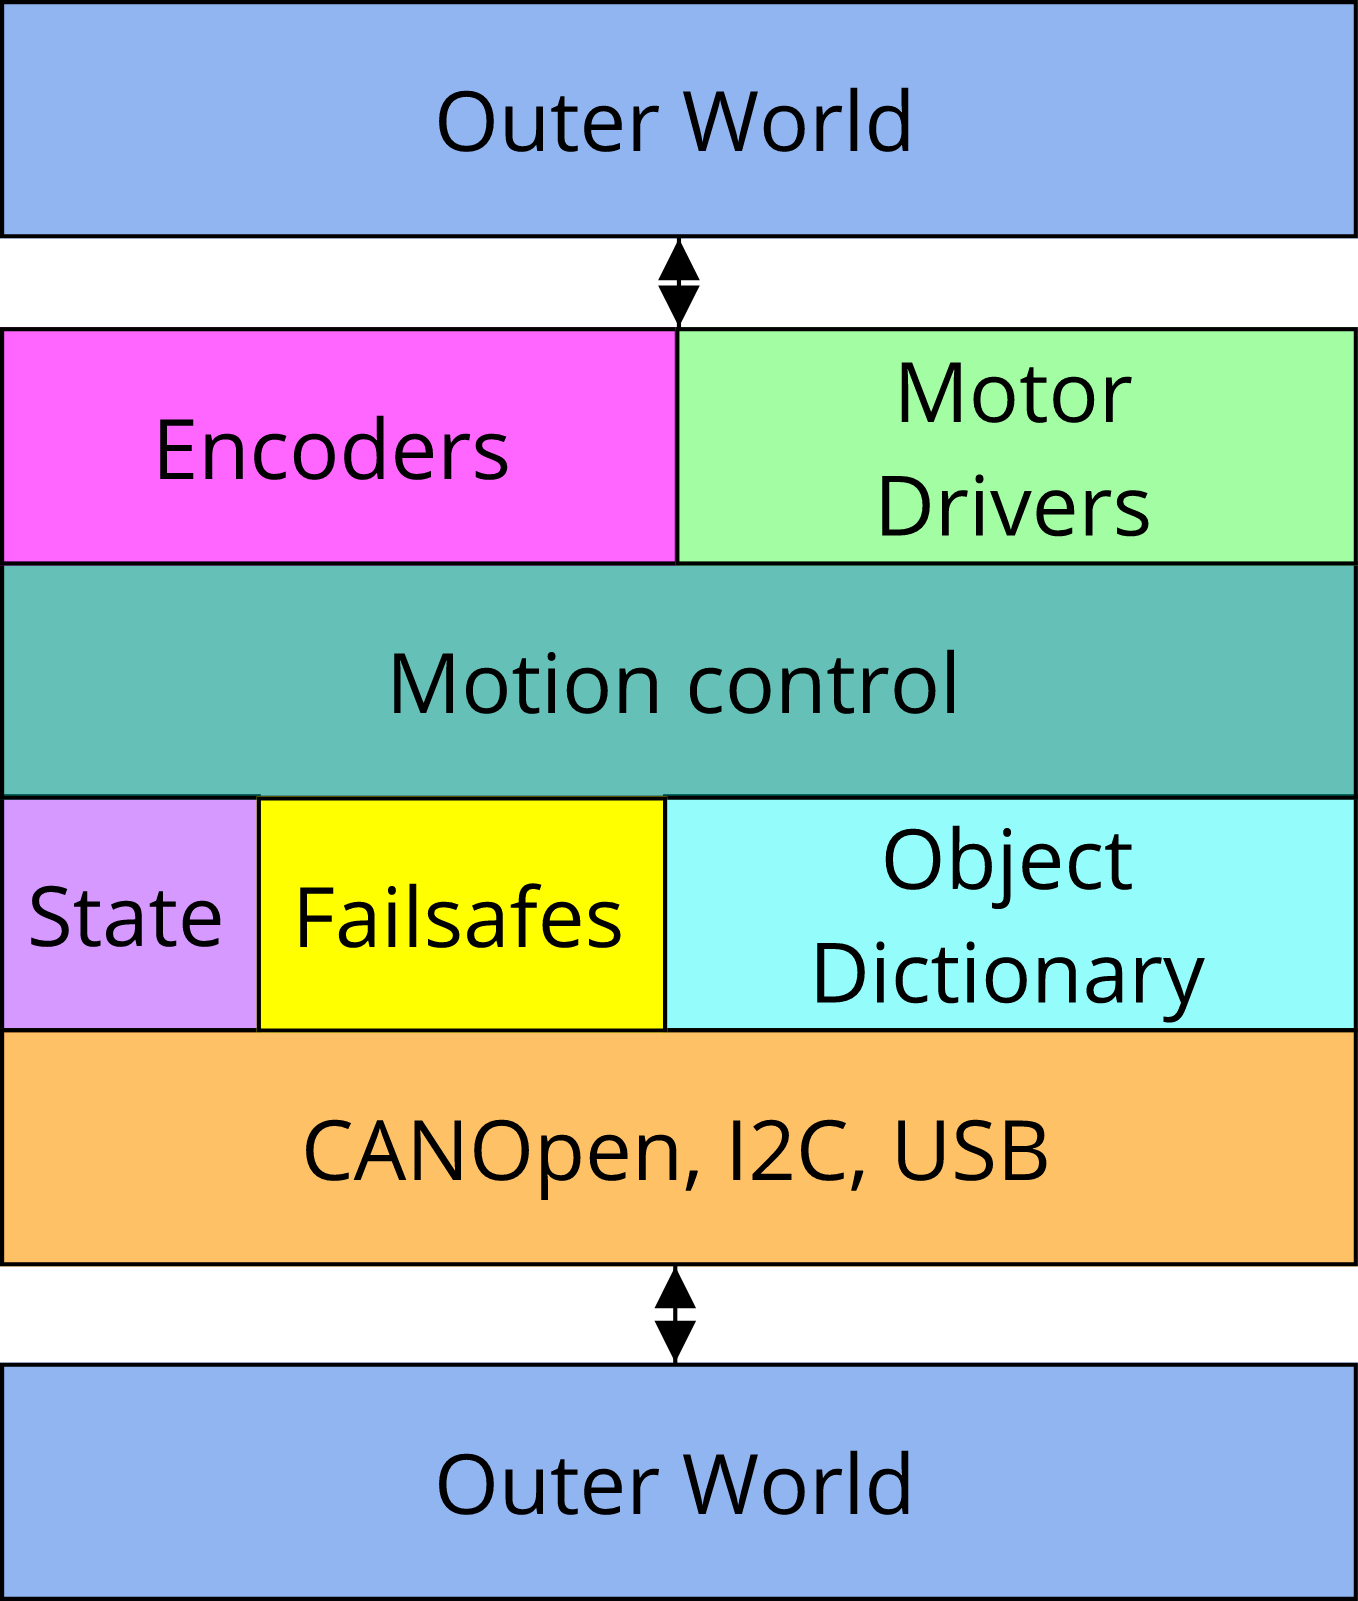
\includegraphics[width=0.5\textwidth]{obrazky/firmware_arch}
    \caption{Bare-Metal firmware technology stack.}
    \label{fig:firmware_arch}
\end{figure}

\subsection{Object Dictionary}
\label{subsec:object_dict_impl}

\subsection{CANOpen Implementation}
\label{subsec:canopen_impl}

\subsection{I2C Implementation}
\label{subsec:i2c_impl}

\subsection{USB}
\label{subsec:usb_impl}

\subsection{Stepper control}
\label{subsec:stepper_control}
Movement of stepper motors, controlled using the stepper motor driver \acs{ic}s is generally controlled using the \textbf{STEP/DIR} interface.
This interface consists of two signals, the first of them named~\textbf{STEP} is a square wave signal with variable frequency, where the edges (rising, falling, or both) instruct the driver to move the motor by a microstep.
On the other hand, the second signal named \textbf{DIR} is generally a logic signal, whose logic level denotes the direction of the shaft movement.

Apart from these two digital signals, there is usually an analog signal that is used to set the motor phase current.
In more modern stepper drivers, this analog signal is replaced by a serial digital interface, allowing for finer current setting.

The \textbf{STEP} signal can be generated either in software (by changing the output logical level of a \acs{gpio} pin) or in hardware by utilizing a \acs{pwm} signal with duty cycle of 50 \%.
Both of these approaches have their limitations and advantages.
Generating the signal in software has the advantage of being able to easily count the number of microsteps the motor was commanded to do, on the other hand the upper limit of the maximal frequency is much lower than with hardware generation and this technique uses more computational resources as the signal is generally generated using an interrupt on timer overflow, where the signal logic level needs to be toggled (which requires branching) and the pulse counter needs to be accessed.
Using a timer with \acs{pwm} allows for much higher maximal frequencies, on the other hand counting the pulses can prove to be quite hard.
This issue will be described in more detail in the Section~\ref{subsec:simulated_encoders}.

We decided to utilize the \textbf{STEP} signal generation done by the hardware as we wanted to offload the work from the \acs{mcu} core.

To abstract the real implementation we created a trait (see Section~\ref{subsec:traits}) for setting the microstepping frequency, as can be seen in the Listing~\ref{lst:step_gen_trait}.
Using this trait the software controlling the stepper driver \acs{ic} can use either hardware or software \textbf{STEP} signal generator.

\begin{lstlisting}[caption={Trait for abstracting STEP generation.},label=lst:step_gen_trait]
/// This trait is an abstraction over hardware/software that is capable of generating square wave signal of specific frequency.
/// It is generally implemented by timers.
pub trait StepGenerator {
    /// Sets output frequency of the generator.
    ///
    /// # Arguments
    /// * `frequency` - frequency of the output square wave signal
    fn set_step_frequency(&mut self, frequency: Hertz);
}
\end{lstlisting}

In our case, the trait is implemented by the abstractions over the \acs{mcu}'s advanced control timers 1 and 8.
The abstractions over the timers are based on the timer implementations that can be found in the \textbf{stm32f4xx-hal}, but are preconfigured to generate output \acs{pwm} signals and also to act as a master timer generating clock signal for other timer on compare.

Using this trait, we were able to define a struct which describes the TMC2100 driver as can be seen in the Listing~\ref{lst:tmc2100}.

\begin{lstlisting}[caption={TMC2100 driver.},label=lst:tmc2100]
pub struct TMC2100<G, STEP, DIR, DAC> {
    generator: G,
    _step_pin: STEP,
    dir_pin: DIR,
    current_dac: DAC,
    sense_r: f32,
    microsteps_per_revolution: f32,
}
\end{lstlisting}
In the Listing, we can see, that the driver contains a generic generator, has ownership of the \textbf{STEP} pin (so that no other peripheral can access it), has ownership of the \acs{DIR} pin, \acs{dac} current reference and knows the value of the sense resistor for current setting and microsteps per revolution for \textbf{STEP} output frequency setting.

For a more seamless integration with the motion controller described in the Section~\ref{subsec:motion_control} the trait \textbf{StepperDriver} was declared as can be seen in the Listing~\ref{lst:stepper_driver_trait}.

\begin{lstlisting}[caption={Trait for abstracting the stepper motor driver IC.},label=lst:stepper_driver_trait]
/// This trait is an abstraction over stepper drivers.
/// Generally the drivers have two functions - generate steps and set output current.
pub trait StepperDriver {
    /// Sets output frequency of the driver.
    /// this shall be the angular frequency of the output shaft in revolutions per second.
    ///
    /// # Arguments
    /// * `frequency` - frequency of the output motor shaft in revolutions per second
    fn set_output_frequency(&mut self, frequency: f32);

    /// Sets the target current the driver shall drive the stepper motor with.
    ///
    /// # Arguments
    /// * `current` - the desired current in Amps
    fn set_current(&mut self, current: f32);
}
\end{lstlisting}

This trait was then implemented for the TMC2100 structure, implementing the stepper control itself, as is shown in the Listing~\ref{lst:stepper_driver_impl}.

\begin{lstlisting}[caption={Implementing the StepperDriver trait for TMC2100.},label=lst:stepper_driver_impl]
impl<G, STEP, DIR, DAC> StepperDriver for TMC2100<G, STEP, DIR, DAC>
where
    G: StepGenerator,
    DIR: embedded_hal::digital::v2::OutputPin,
    DAC: DACChannel,
{
    fn set_output_frequency(&mut self, frequency: f32) {
        if frequency < 0.0 {
            self.dir_pin.set_high().ok();
        } else {
            self.dir_pin.set_low().ok();
        };
        self.generator.set_step_frequency(Hertz::new(
            (frequency.abs() * self.microsteps_per_revolution) as u32,
        ))
    }
    fn set_current(&mut self, current: f32) {
        let voltage =
            (current.abs() * MAX_V_REF as f32 / V_FS * (self.sense_r + R_OFFSET) / 0.707) as u16;
        self.current_dac.set_output_voltage(voltage.min(MAX_V_REF));
    }
}
\end{lstlisting}

\subsection{Simulated encoders}
\label{subsec:simulated_encoders}

\subsection{Device Monitoring}
\label{subsec:device_monitoring}
In order to provide status and health information, simple device monitoring is employed.
The monitoring system periodically reads internal \acs{mcu} temperature and the motor voltage.
This functionality is implemented by accessing the internal \acs{mcu} \acs{adc}.
The internal \acs{adc} utilizes the Successive approximation principle and supports up-to 19 channels\cite{stmicro_stm32f405xx_2020}.
The \acs{adc} is configured to read the two channels and to use \acs{dma} to transfer the values from the peripheral to the program's memory.
Both \acs{adc} configuration and \acs{dma} transfer are already implemented in the \textbf{stm32f4xx-hal} crate, meaning that no low-level peripheral access code was required.
The monitoring data are periodically transferred to the Object Dictionary by the higher-level code.

First, we configure the \acs{adc} as can be seen in the Listing~\ref{lst:adc}.
We set the \acs{dma} transfer mode to \textbf{Continuous} (which reissues a \acs{dma} request on every start of conversion) and enable scan mode, which scans all the channels in the sequence.
Further, both of the channels are configured, with assignment to pin/ or special channel, order in the conversion sequence and sample time, which denotes for how many clock cycles the sample-and-hold circuits samples.
Finally, the temperature and VRef channel measurement is enabled as it is not enabled by default by the hardware.

\begin{lstlisting}[caption={Configuring ADC for temperature and voltage monitoring.},label=lst:adc]
let mut adc = Adc::adc1(raw_adc, true, adc_config);
let adc_config = AdcConfig::default()
     .dma(Dma::Continuous)
     .scan(Scan::Enabled);
adc.configure_channel(&Temperature, Sequence::One, SampleTime::Cycles_480);
adc.configure_channel(&battery_voltage, Sequence::Two, SampleTime::Cycles_480);
adc.enable_temperature_and_vref();
\end{lstlisting}

Next, we configure the \acs{dma} transfer, as can be seen in the Listing~\ref{lst:dma}.
We configure the \acs{dma} controller to issue an interrupt when the transfer is complete, to increment addresses only in memory and not in the peripheral and we disable double buffering.

\begin{lstlisting}[caption={Configuration of the DMA controller for ADC transfers.},label=lst:dma]
let first_buffer = singleton!(: [u16; 2] = [0; 2]).unwrap();
let config = DmaConfig::default()
    .transfer_complete_interrupt(true)
    .memory_increment(true)
    .double_buffer(false);
let transfer = Transfer::init(dma, adc, first_buffer, None, config);
\end{lstlisting}

The monitoring system is then periodically asked to poll data from the \acs{adc} by starting the transfer as can be seen in the following Listing~\ref{lst:adc_poll}.
\begin{lstlisting}[caption={Polling the ADC.},label=lst:adc_poll]
self.transfer.start(|adc| {
    adc.start_conversion();
});
\end{lstlisting}
When the \acs{dma} transfer complete interrupt routine is called, the next transfer is prepared and the measured data is processed using factory calibration and formulae that can be found in the reference manual\cite{stmicro_stm32f405xx_2020}.
The final two coefficients in the battery\_voltage calculation represent the voltage divider described in the Section~\ref{subsec:aux_connectors}.
The preparation and calculation is shown in the Listing~\ref{lst:adc_isr}.
\begin{lstlisting}[caption={Processing the data measured by the ADC.},label=lst:adc_isr]
let (buffer, _) = self
    .transfer
    .next_transfer(self.buffer.take().unwrap())
    .unwrap();
let raw_temp = buffer[0];
let raw_volt = buffer[1];
self.buffer = Some(buffer);
let cal30 = VtempCal30::get().read() as f32;
let cal110 = VtempCal110::get().read() as f32;
self.temperature = (110.0 - 30.0) * ((raw_temp as f32) - cal30) / (cal110 - cal30) + 30.0;
self.battery_voltage = (raw_volt as f32) / ((2_i32.pow(12) - 1) as f32) * 3.3 / 4.7 * 104.7;
\end{lstlisting}

\subsection{Motion Control}
\label{subsec:motion_control}
% psd, ramping

\begin{figure}[H]
    \centering
    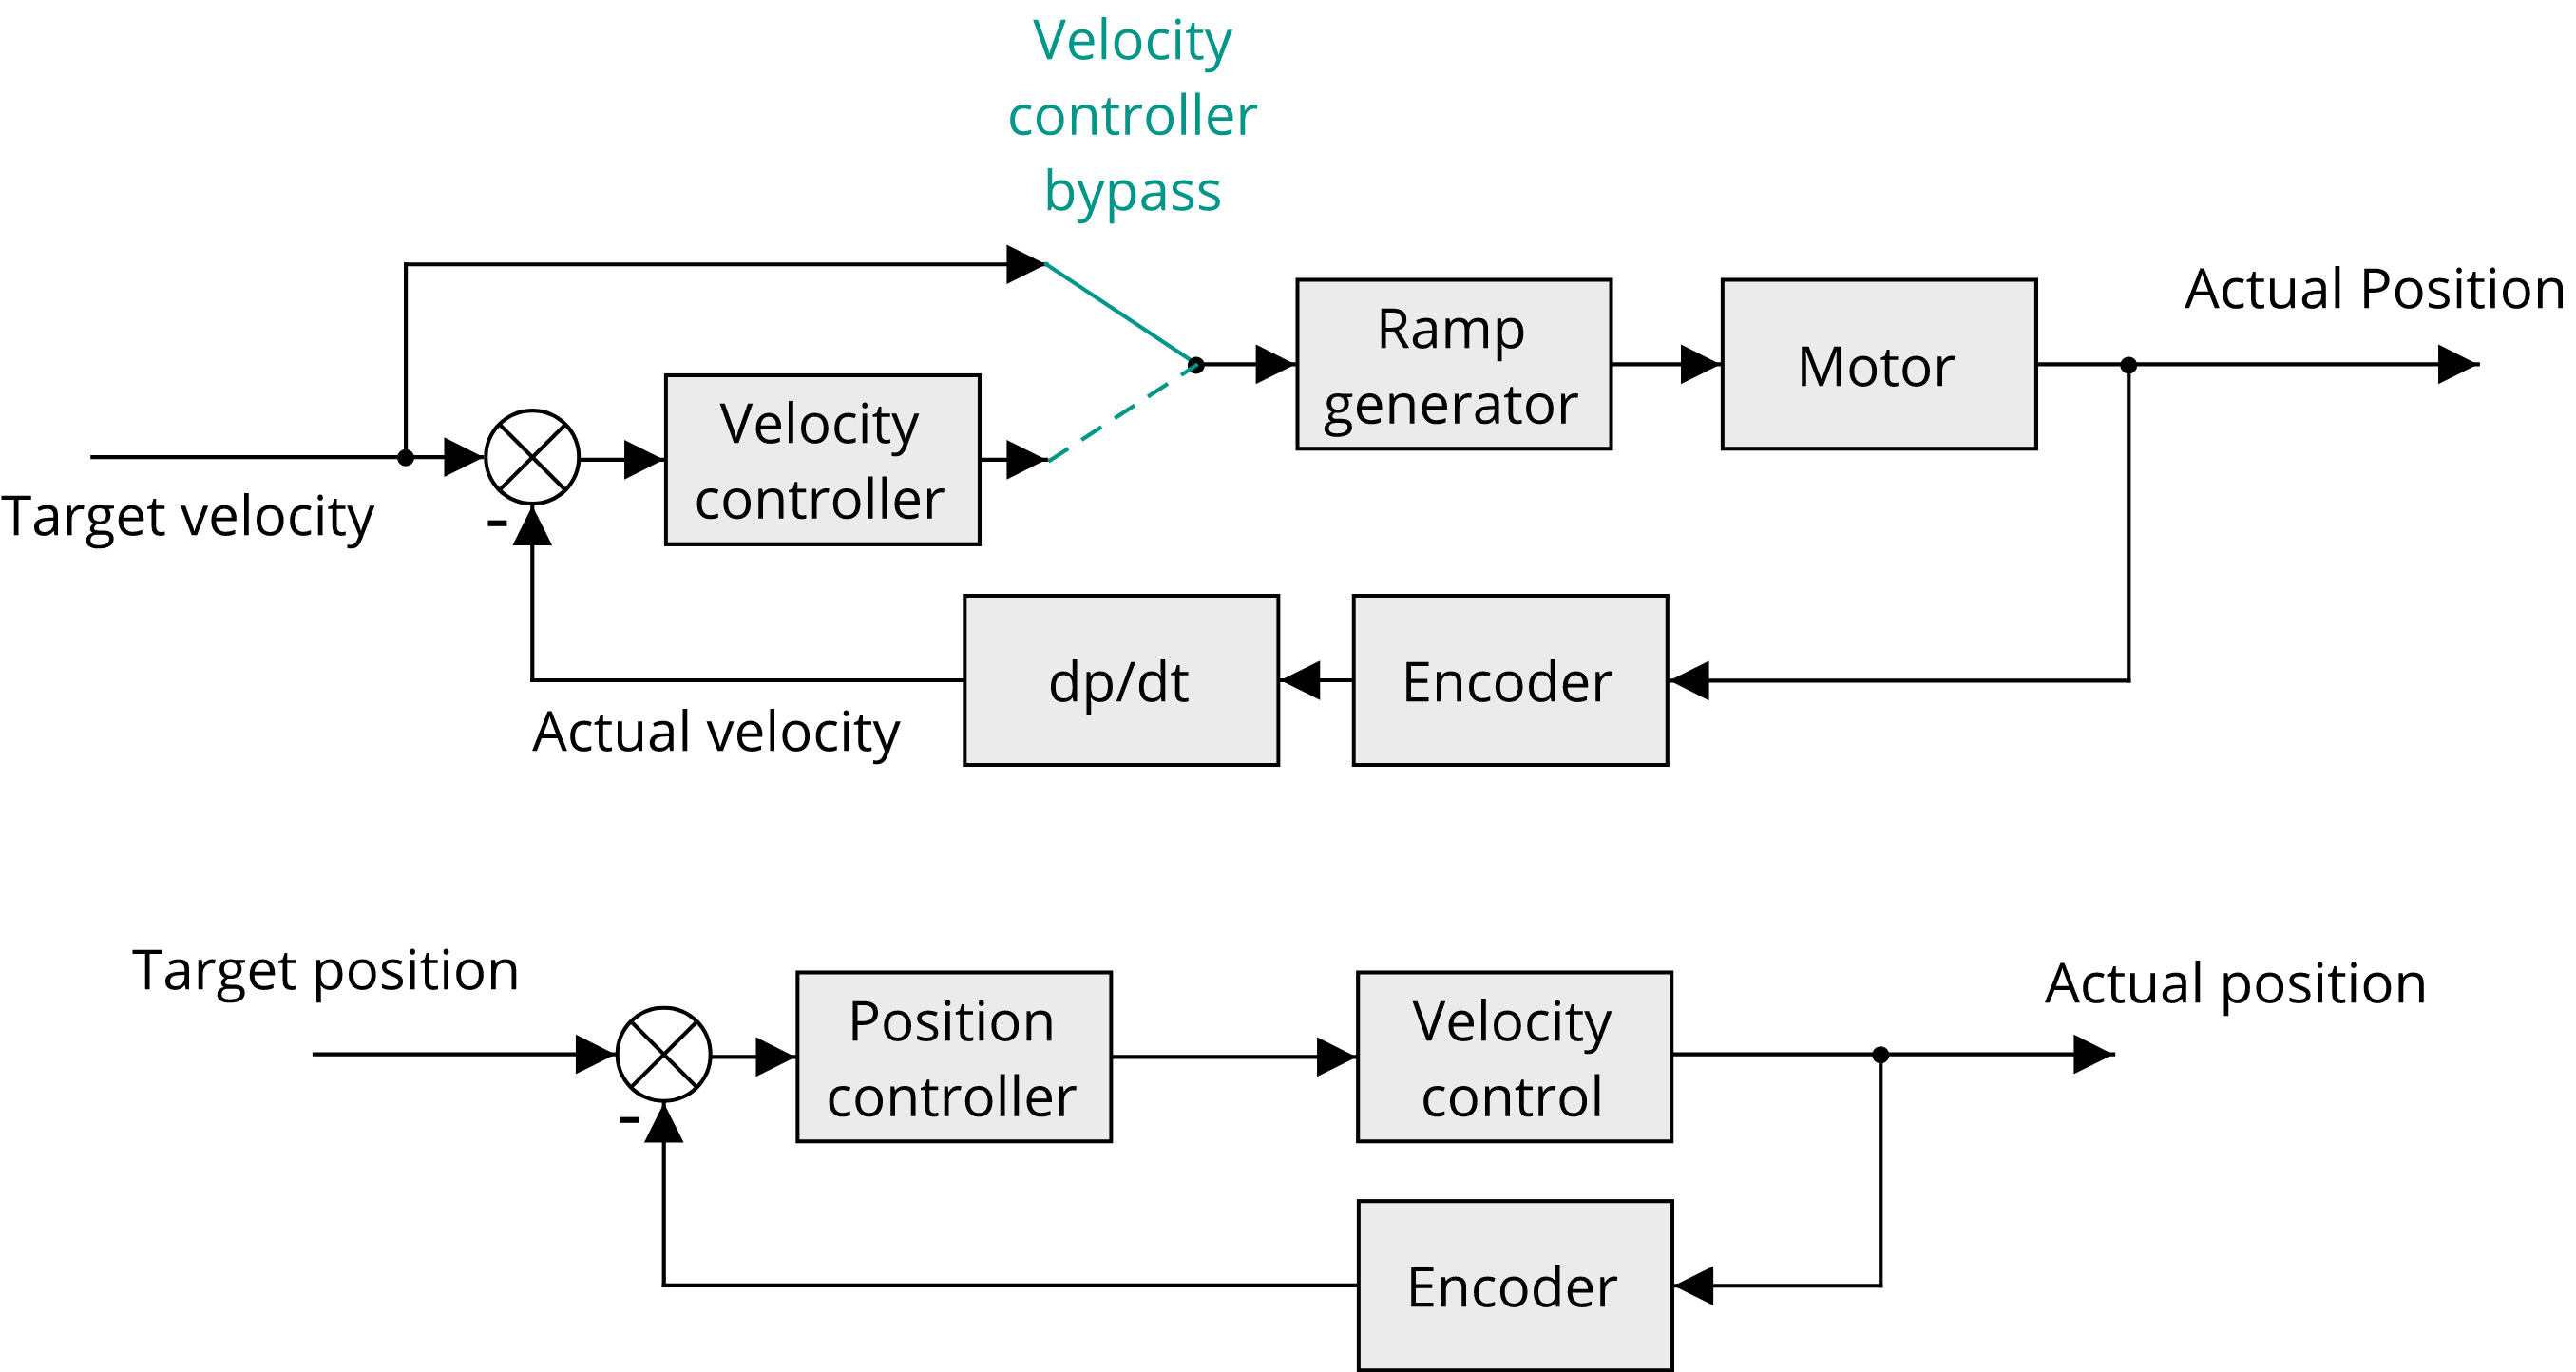
\includegraphics[width=\textwidth]{obrazky/motion_control}
    \caption{Motion control schematic.}
    \label{fig:motion_control}
\end{figure}
